\documentclass[14pt]{article}

\usepackage[utf8]{inputenc}
\usepackage[T1]{fontenc}
\usepackage{extsizes}
\usepackage[english,russian]{babel}
\usepackage{geometry}
\usepackage{tempora}
\usepackage{amsmath}
\usepackage{graphicx}
\usepackage{hyperref}
\usepackage{listings}
\usepackage{xcolor}
\usepackage{scrextend}
\usepackage{float}

\geometry{
    a4paper,
    left=30mm,
    top=20mm,
    right=20mm,
    bottom=20mm
}

\definecolor{dkgreen}{rgb}{0,0.6,0}
\definecolor{gray}{rgb}{0.5,0.5,0.5}
\definecolor{mauve}{rgb}{0.58,0,0.82}

\lstdefinestyle{scalaStyle}{
  frame=tb,
  language=scala,
  aboveskip=3mm,
  belowskip=3mm,
  showstringspaces=false,
  columns=flexible,
  basicstyle={\small\ttfamily},
  numbers=none,
  numberstyle=\tiny\color{gray},
  keywordstyle=\color{blue},
  commentstyle=\color{dkgreen},
  stringstyle=\color{mauve},
  frame=single,
  breaklines=true,
  breakatwhitespace=true,
  tabsize=3,
}

\linespread{1.5}

\begin{document}
\begin{titlepage}
    \begin{center}
        Министерство образования и науки Российской Федерации\\
        \vspace{4mm}
        Государственное образовательное учреждение высшего профессионального образования <<Московский физико-технический институт (государственный университет)>>\\
        \vspace{4mm}
        Физтех-школа прикладной математики и информатики\\
        \vspace{4mm}
        Кафедра корпоративных информационных систем\\
        \vspace{4mm}
        Выпускная квалификационная работа по направлению 03.03.01 Прикладные
математика и физика (бакалавриат)
        \vfill
        {\LARGE \textbf{Эффективная классификация событий в потоковых системах}}\\
        \vfill
        \begin{addmargin}[4cm]{0cm}
        \textbf{Студент}: Валентинов Александр Александрович\\
        \textbf{Научный руководитель}: Шеронова Анна Николаевна
        \end{addmargin}
        \vfill
        г. Москва, 2020
    \end{center}
\end{titlepage}

\clearpage
\tableofcontents
\clearpage
\section{Вступление}
Потоковые системы или системы, ориентированные на обработку сообщений, являются одним из широко используемых подходов для работы с большим объемом данных. Они предоставляют множество преимуществ: возможность асинхронной обработки сообщений повышает надежность и сохранность данных, а способность транслировать сообщения нескольким получателям способствует их переиспользованию.

Часто сообщения в потоковых системах представляют некоторые бизнес-события. Одна из задач, возникающих при работе с потоковыми системами --- задача классификации этих бизнес-событий: из потока необходимо выделить события, которые удовлетворяют некоторым правилам. Если правил достаточно много, то наивное решение с сопоставлением всех событий всем правилам начинает работать недостаточно быстро. Эта работа посвящена решению данной проблемы.

\section{Анализ задачи}
\subsection{Определения}
Введем несколько определений, необходимых для формальной постановки задачи.
Ниже будем считать, что количество признаков (длина кортежей) $d$ --- это некоторое <<небольшое>> целое число.
В данной работе считается, что $d$ находится в пределах $[1, 32]$.

\emph{Событие} --- кортеж длины $d$ из чисел в пределах $[0, 1]$: $X = (x_1,\ldots,x_d), \forall i: x_i \in [0, 1]$.

\emph{Правило} --- кортеж длины $d$ из предикатов $P = (p_1,\ldots,p_d), \forall i: p_i(x): [0, 1] \rightarrow \{0, 1\}$, каждый из которых имеет один из видов:
\begin{itemize}
    \item $p_i(x) \equiv 1$;
    \item $ p_i(x) =
        \begin{cases}
        1, & a \leq x \leq b, \\
        0, & a > x \vee x > b.
        \end{cases}
    $ --- для некоторых фиксированных $a$ и $b$, $0 \leq a \leq b \leq 1$;
    \item $ p_i(x) =
        \begin{cases}
        1, & a \leq x, \\
        0, & a > x.
        \end{cases}
    $ --- для некоторого фиксированного $a$, $0 \leq a \leq 1$;
    \item $ p_i(x) =
        \begin{cases}
        1, & x \leq b, \\
        0, & x > b.
        \end{cases}
    $ --- для некоторого фиксированного $b$, $0 \leq b \leq 1$;
    \item $ p_i(x) =
        \begin{cases}
        1, & x = a, \\
        0, & x \neq a.
        \end{cases}
    $ --- для некоторого фиксированного $a$, $0 \leq a \leq 1$.
\end{itemize}

\emph{Совпадение} --- пара из события и правила, такое что каждый элемент кортежа-события удовлетворяет соответствующему предикату из правила: $(X, P): \prod_{i=1}^d p_i(x_i) = 1$.

\subsection{Постановка задачи}
Имеется поток событий, которые можно читать из некоторой входной очереди сообщений. Также есть набор правил, который хранится в базе данных. Необходимо находить все совпадения между событиями и правилами так, чтобы за единицу времени обрабатывалось как можно больше событий, и записывать результаты в выходную очередь.

Количество событий, появляющихся во входной очереди может быть больше, чем возможно эффективно обработать на одном сервере, поэтому система должна быть горизонтально-масштабируемой. Ориентировочные значения нагрузки --- тысячи событий в секунду и десятки тысяч правил.

Набор правил может изменяться, но допускается задержка в обработке изменений правил. Это допущение необходимо для того, чтобы система, решающая задачу, могла строить неизменяемые индексы.

Задача этой работы --- спроектировать систему, решающую эту задачу и реализовать ее прототип.

\subsection{Возможные применения и мотивация}
Задача встречается, когда широкому кругу пользователей необходимо выделить интересующие их события из потока бизнес событий. Ниже несколько примеров:
\begin{itemize}
    \item У агрегатора интернет-магазинов есть поток бизнес-событий вида <<Товар $A$ марки $B$, с характеристиками $C$, $D$, и $E$, ценой $F$ появился в магазине $G$>>. Используя систему, решающую задачу классификации событий, пользователь может подписаться на появление какого-то товара, создав правило, с интересующими его параметрами. Пример такого правила --- <<\emph{Чайник} марки \emph{Panasonic} \emph{зеленого цвета}, ценой от \emph{1000 рублей} появился в \emph{любом} магазине>>. Нечисловые параметры можно кодировать числами на входе и выходе из системы.
    \item Поисковик авиабилетов записывает в очередь результаты поисков в виде <<Билет из аэропорта $A$ в аэропорт $B$, с $C$ пересадками ценой $D$>>. С помощью системы пользователь может следить за ценами на интересующие его авиабилеты, создав правило, например =<<Билет из \emph{Пекина} во \emph{Францию} с \emph{не более, чем двумя} пересадками, \emph{не дороже 20000 рублей}>>. Страну в правиле можно представить как отрезок чисел, а аэропорты --- числами в этом отрезке.
\end{itemize}

Главное достоинство такой системы --- возможность анализировать события, не сохраняя их на долгое время и не запуская какие-то процессы, которые бы для каждого правила искали подходящие события.

\subsection{Анализ аналогов}
Существующие аналоги для решения задачи классификации можно разбить на две группы: фреймворки для обработки потоковых данных и базы данных, имеющие возможность хранить пространственные данные.

Фреймворки для обработки потоковых данных, среди которых, например Apache Flink, Apache Storm, Apache Samza и другие, больше рассчитаны на подсчет агрегатов~\cite{flink-use-cases, storm-documentation, samza-streams-api}, чем на сопоставление событий из потока с правилами. Используя стандартные функции этих фреймворков, возможно реализовать решение этой задачи, но при большом числе правил оно будет не так эффективно, как расмотренное в этой работе. К тому же, многие из таких фреймворков нацелены на offline-обработку, в нашем случае необходима online-обработка событий. Способы решения задачи, которые будут описаны в следующих главах, можно интегрировать с такими фреймворками, но, для упрощения реализации, они не используются.

Базы данных, имеющие возможность работать с пространственными данными --- MySQL, PostgreSQL + PostGIS, Oracle Spatial и т.п. позволяют хранить многомерные данные, но они оптимизированы для задач, связанных с обработкой геоданных --- двумерных координат на карте Земли~\cite{mysql-spatial, postgis, oracle-spatial}. При работе с многомерными данными они либо неприменимы, либо неэффективны.

\section{Архитектура}
\subsection{Архитектура в случае одного сервера}
Сначала будут рассмотрены возможные варианты архитектуры системы, при наличии всего одного сервера. Будет сравнено наивное решение и несколько вариантов индексов.

\subsubsection{Наивное решение}
В случае наивного решения правила читаются из базы и кешируются на определенное время. После истечения этого времени они снова читаются и кешируются, чтобы получить изменения, которые, возможно, произошли в правилах.

События читаются из входной очереди по одному и сопоставляются с каждым из правил. Если находятся совпадения, они записываются в выходную очередь по одному. Пусть $|P_\alpha|$ --- количество правил. Так как используется линейный поиск, сложность нахождения всех правил для одного события --- $O(|P_\alpha|)$. Для $n$ правил сложность составляет $O(n|P_\alpha|)$.

\subsubsection{R-деревья}
Во всех решениях, описанных ниже, используются различные вариации $R$-деревьев~\cite{r-tree}. Это специальный вид деревьев, который позволяет индексировать многомерные точки и прямоугольники. Каждый узел $R$-дерева имеет не более максимально допустимого числа детей и хранит ограничивающий прямоугольник для объектов или поддеревьев, которые в нем содержатся. Основная идея работы $R$-дерева состоит в том, что оно разбивает пространство на множество иерархически вложенных многомерных прямоугольников, которые, возможно, пересекаются между собой. Это позволяет группировать <<близкие>> объекты по узлам и листьям дерева и увеличивает эффективность поиска.

К $R$-дереву можно делать запросы как на поиск всех прямоугольников, которые содержат заданную точку, так и на поиск всех точек, которые находятся в заданном прямоугольнике. Второй тип запросов работает медленнее, т.к. приходится проверять больше вершин.

Для вставки одного объекта необходимо использовать эвристику, которая определяет, какой узел нужно выбрать для вставки и как, при необходимости, разбить узел. Большинство эвристик хорошо работают только для вставки в случае двумерного пространства.

\paragraph{X-дерево.} Наиболее эффективным вариантом $R$ дерева для работы с многомерными данными является $X$-дерево~\cite{x-tree}. Оно использует алгоритм выбора и разбиения основанный на алгоритме $R^*$-дерева~\cite{r-star-tree}. При разбиении узла, если эвристика $R^*$-дерева дает результат со слишком большим пересечением ограничивающих прямоугольников, сначала происходит попытка разбить узел, основываясь на истории предыдущих разбиений. Если вторая попытка разбить узел также дает слишком большое пересечение, узел не разбивается, превращаясь в супер-узел с числом детей, большим, чем максимально допустимое. Это позволяет избегать неоптимальных разбиений и уменьшает количество посещаемых поддеревьев поиск более эффективным. Амортизированная сложность вставки в $X$-дерево с $n$ элементами и максимальным числом элементов в узле равном $M$ --- $O(\log_M n)$. Вставка $n$ элементов будет иметь сложность $O(n\log_M n)$.

\paragraph{Алгоритм массовой вставки в R-дерево.} Другой способ построить оптимальное $R$-дерево в случае многомерного пространства --- алгоритм массовой вставки в $R$-дерево~\cite{str, omt}. Он применим, когда заранее известны все объекты, которые нужно вставить в дерево. Алгоритм начинает работу из корня будущего дерева. На каждом шаге рассчитывается, сколько детей будет у узла, который сейчас создается --- $s$ (если узел не является корнем, то это число равно максимальному числу детей у узла). Далее все объекты сортируются по началу отрезка ограничивающего прямоугольника в измерении $h\mod d$, где $h$ --- глубина создаваемого узла (для корня --- 0, для ребенка корня --- 1 и т.д.). Потом отсортированный массив объектов разбивается на $s$ групп. Каждая группа --- объекты, которые содержатся в одном из поддеревьев корня. Затем алгоритм рекурсивно запускается для каждой из этих групп. В результате получается сбалансированное дерево, в котором ограничивающие прямоугольники слабо пересекаются. В случае, если в дерево записываются только точки, ограничивающие прямоугольники не пересекаются совсем. Сложность построения $R$-дерева алгоритмом массовой вставки --- $O(n\log n)$.

Из-за того, что в результате применения этих двух подходов получаются хорошо сбалансированные $R$-деревья, они позволяют достаточно эффективно индексировать как точки, так и многомерные прямоугольники. Сложность чтения из сбалансированного $R$-дерева --- $O(\log_M n)$, где $M$ --- максимальное допустимое число элементов в узле, а $n$ --- количество элементов в дереве.

\subsubsection{Подходы к индексированию}
\label{section:indexingApproaches}
Для задачи классификации можно использовать два способа. Первый способ --- индексировать правила и искать в этом индексе точки по одной. Второй --- группировать события во входном потоке, строить по группе индекс и искать в этом индексе все правила.

Чтобы применять индексы к задаче классификации, необходимо определить отображение между правилами и многомерными прямоугольниками. Преобразования между предикатами и отрезками определяются следующим образом:
\begin{itemize}
    \item $a \leq x \leq b \quad \simeq \quad [a ,b]$
    \item $a \leq x \quad \simeq \quad [a, 1]$
    \item $x \leq b \quad \simeq \quad [0, b]$
    \item $ x = a \quad \simeq \quad [a, a]$
    \item $ x = x \quad \simeq \quad [0, 1]$
\end{itemize}
Например, правило $(x_1 \leq 0.1, 0.6 \leq x_2, 0.5 \leq x_3 \leq 0.7, x_4 = 0.2, x_5 = x_5)$ преобразуется в прямоугольник $[0, 0.1]\times[0.6, 1]\times[0.5, 0.7]\times[0.2, 0.2]\times[0, 1]$.

\paragraph{Индексация правил.} При данном подходе каждое правило преобразуется в прямоугольник и на этих прямоугольниках строится $R$-дерево. Используя алгоритм поиска точки в $R$-дереве, можно найти все правила, которым удовлетворяет событие. При таком подходе правила хранятся в дереве. События читаются из входной очереди по одному. Для каждого события ищутся все правила, под которые оно подходит. Найденные совпадения записываются в выходную очередь. Через определенный промежуток времени правила читаются из базы и индекс перестраивается, чтобы учитывать изменения, которые могли произойти в правилах.

Сложность поиска одного события в $R$-дереве с $n$ прямоугольниками --- $O(\log n)$. Сложность обработки $k$ событий равна
\[O(k \log n).\]

\begin{figure}[h]
  \centering
    \includegraphics[width=1\textwidth]{RulesArch.png}
  \caption{Индексация правил.}
\end{figure}

\paragraph{Индексация событий.} В этом подходе к индексации события читаются из входной очереди группами фиксированного размера. Из каждой группы строится $R$-дерево. Правила читаются из базы и преобразуются в многомерные прямоугольники, результат кешируется. C помощью алгоритма поиска всех точек, входящих в заданный прямоугольник, в $R$-дереве ищутся все точки, которые удовлетворяют каждому правилу. Найденные совпадения записываются в выходную очередь.

Построение дерева по группе точек размера $g$ имеет сложность $O(g\log g)$. Сложность поиска одного правила --- $O(\log g)$, поиска $n$ правил --- $O(n\log g)$. Итого, сложность обработки одной группы --- $O(g\log g + n\log g)$. Сложность обработки $k$ событий будет равна
\[ O\left(\frac{k}{g}(g\log g + n\log g)\right) = O\left(\left(k + \frac{n}{g}\right)\log g\right).\]

\begin{figure}[h]
  \centering
    \includegraphics[width=1\textwidth]{PointsArch.png}
  \caption{Индексация событий.}
\end{figure}

\paragraph{Сравнение эффективности подходов.} $R$-деревья, в которых хранятся только точки, имеют более оптимальную для запросов на поиск структуру, потому что точки легче разбить на непересекающиеся группы. Это делает поиск в подходе с индексацией событий более эффективным. С другой стороны, при этом подходе необходимо заново строить индекс для каждой группы событий, что ведет к большому количеству аллокаций. Использование подхода с индексацией правил позволяет строить индекс один раз, не учитывая кеширования. Сравнение подходов на практике, а также подбор оптимального значения константы $g$ для подхода с индексацией событий, будет описан в главе <<\nameref{section:testing}>>.

\subsection{Общая архитектура системы}
\label{section:commonArch}
В отличие от архитектуры в случае одного сервера, для работы всей системы необходимо добавить логику для масштабирования. Масштабировать систему можно относительно двух параметров: количества правил и количества событий, поступающих в единицу времени.

В случае, если растет количество правил, могут возникать сложности с хранением всех правил в индексе на одном сервере. Например, будет заканчиваться оперативная память, расходуемая на хранение правил в индексе или на запись в очередь большого количества совпадений. Для решения этой проблемы можно разбить правила между несколькими серверами, так, что на одном сервере будет храниться только часть правил.

При росте количества поступающий событий, пропускной способности одного сервера может не хватить для обработки всех событий. В таком случае события начнут накапливаться в очереди и, рано или поздно, займут все доступное для хранения место. Решить эту проблему можно аналогично предыдущему случаю: разбив события между серверами. Таким образом, один сервер будет получать только часть всех событий.

Если скомбинировать решения проблем масштабирования при росте числа правил и при росте количества событий за единицу времени, получится, что каждый сервер должен индексировать только часть правил о обрабатывать только часть запросов. Достигнуть этого можно разбив сервера на группы. Каждая группа получает равную долю правил, и все события. Каждый сервер внутри группы обрабатывает свою часть событий. Схема разделения правил и событий изображена на рисунке~\ref{fig:commonArch}.

Для распределения правил и событий необходим некоторый сервис координации, через который будут синхронизироваться сервера с индексами. Таким образом, общий список необходимых сервисов будет выглядеть так:
\begin{itemize}
    \item Входная очередь --- для получения событий;
    \item База данных --- для хранения правил;
    \item Сервис координации --- для распределения правил и событий между серверами, производящими поиск совпадений;
    \item Сервера, производящие поиск совпадений;
    \item Выходная очередь --- для сохранения совпадений.
\end{itemize}
Кроме того, вне системы есть еще несколько необходимых сервисов, которые непосредственно не участвуют в поиске совпадений:
\begin{itemize}
    \item Источник событий --- сервис, который производит события и сохраняет их во входную очередь;
    \item Обработчик совпадений --- сервис, который читает совпадения из выходной очереди и обрабатывает их так, как необходимо пользователю;
    \item Интерфейс к базе данных --- сервис, через который можно создавать правила и сохранять их в базу.
\end{itemize}
Необходимые сервисы представлены на рисунке~\ref{fig:commonArch}.

\begin{figure}[h]
  \centering
    \includegraphics[width=1\textwidth]{CommonArch.png}
    \caption{Общая архитектура системы.}
    \label{fig:commonArch}
\end{figure}

\section{Разработка и развертывание}
В этой главе будут рассмотрены технологии, которые использовались при разработке прототипа системы, будут объяснены причины выбора этих технологий и рассмотрены ключевые моменты реализации сервисов.

\subsection{Выбор технологий}
\subsubsection{Очереди}
В качестве очереди, или, точнее, брокера сообщений используется Apache Kafka~\cite{kafka}. Apache Kafka способна эффективно обрабатывать большое количество сообщений. Механизм топиков (topics) позволяет работать с несколькими очередями, используя один кластер. Благодаря группам потребителей (consumer groups) возможно удобно реализовать разделение событий между серверами внутри одной группы, как описано в главе~\ref{section:commonArch}. Потребители, находящиеся в одной группе потребителей разделяют сообщения, получаемые из топика. Несмотря на преимущества этого подхода, у него есть один недостаток: количество потребителей в группе ограничено количеством партиций (partitions) в топике. При разработке системы необходимо учесть этот факт. Это будет подробнее описано в главе~\ref{section:classifier}.

\subsubsection{Сервис координации}
Для координации серверов, которые ищут совпадения, используется Apache ZooKeeper~\cite{zookeeper}. Apache ZooKeeper --- надежный сервис, который позволяет реализовывать множество различных протоколов синхронизации. Для упрощения работы с Apache ZooKeeper существует клиентская библиотека Apache Curator~\cite{curator}. Она используется в приложениях для поиска совпадений. Кроме того, ZooKeeper необходим для работы ApacheKafka. Его можно переиспользовать и для распределения правил между индексами.

\subsubsection{База данных}
В роли базы данных для хранения правил выступает MongoDB~\cite{mongo}. MongoDB --- простая в использовании документоориентированная база данных. Она предоставляет достаточную производительность для системы классификации событий. Для системы подойдет любая база данных, которая поддерживает редкие запросы на чтение большого диапазона записей и способна хранить достаточное количество данных.

\subsubsection{Сервисы системы классификации}
Сервисы системы классификации --- это сервис для создания событий, сервис для поиска совпадений и сервис для их валидации. Первый и последний сервисы непосредственно не входят в системы классифиации, но используются при ее тестировании. Для разработки этих сервисов используется язык программирования Scala~\cite{scala}, так как, с одной стороны, он предоставляет удобные функциональные абстракции для работы с данными, а с другой поддерживает интеграцию с Java, что позволяет использовать многие библиотеки из экосистемы этого языка. Основные используемые абстракции и библиотеки описаны в главе~\ref{section:scalaAbstractions}.

\subsubsection{Мониторинг}
При тестировании системы необходимо собирать данные о работе всех серверов и визуализировать их в одном месте. Для решения этой задачи используется Prometheus~\cite{prometheus} (сбор метрик) и Grafana~\cite{grafana} (визуализация).

\subsubsection{Развертывание}
Для развертывания всех сервисов используется Docker~\cite{docker}. Docker позволяет запускать приложение и необходимое окружение в легковесном контейнере (container). Несколько изолированных контейнеров могут быть запущены на одном физическом сервере, при этом они делят операционную систему, что делает использование Docker более эффективным, чем использование виртуальных машин. Один Docker-контейнер обычно соответствует одному запущенному экземпляру приложения.

Docker-контейнеры создаются из специальных образов (image), в которых описано, как запустить нужное приложение, и какие зависимости ему нужны. Для всех сервисов, используемых при разработке системы существуют заранее определенные Docker-образы. Для сервисов системы классификации Docker-образы создаются средствами инструметнов сборки Scala.

Docker предоставляет удобные инструменты для запуска нескольких контейнеров, образующих одну систему как на одном физическом сервере (Docker Compose), так и на нескольких физических серверах (Docker Swarm Mode). Для этого используется специальный файл \verb|docker-compose.yml|, в котором указываются все необходимые связи между сервисами и параметры окружения.

\subsection{Разработка}
\subsubsection{Основные абстракции Scala}
\label{section:scalaAbstractions}
В приложениях используются две основные абстракции: эффект (effect) и поток (stream).

\emph{Эффект} --- это абстракция, которая описывает вычисления, имеющие сторонние эффекты и потенциально асинхронные. В Scala эффект --- это обычно полиморфный тип \verb|F[A]|, запустив экземпляр которого, можно получить значение типа \verb|A|. Можно провести аналогию между Scala-эффектом и \verb|Promise| в JavaScript и \verb|Future| в Java, только Scala-эффект является ленивым, то есть исполняется только при получении явной команды на исполнение.

Для работы с эффектами в сервисах системы классификации используется библиотека ZIO~\cite{zio}. В коде эффекты обозначаются типом \verb|ERIO[_]|.

\emph{Поток} --- это абстракция описывает потоки данных и позволяет производить над ними различные операции: изменять элементы, группировать, агрегировать и тому подобные.

Для работы с потоками используется библиотека Functional Streams For Scala~(fs2)~\cite{fs2}. В коде поток данных представляется типом \verb|Stream[ERIO, _]|.

\subsubsection{Основные модели данных}
Ниже описаны ключевые модели данных.
\paragraph{Событие.} Событие представляется классом \verb|Point| (листинг~\ref{listing:point}), который является оберткой над вектором чисел с плавающей точкой. Длина этого вектора --- количество измерений --- должна быть согласована между сервисами.

\begin{lstlisting}[style=scalaStyle,caption={Класс, описывающий событие.},label={listing:point},captionpos=b, float]
final case class Point(values: Vector[Double])
\end{lstlisting}

\paragraph{Правило.}
Правило представляется типом \verb|Rule| (листинг~\ref{listing:rule}), который является синонимом для вектора экземпляров интерфейса \verb|Restriction| --- возможных ограничений на каждое из измерений события. Длина этого вектора также должна быть согласована с между сервисами и с количеством измерений в событии.

\begin{lstlisting}[style=scalaStyle,caption={Тип, описывающий правило.},label={listing:rule},captionpos=b, float]
type Rule = Vector[Restriction]

sealed trait Restriction
final case class Exact(value: Double) extends Restriction
final case class Interval(from: Double, to: Double) extends Restriction
final case class Less(to: Double) extends Restriction
final case class Greater(from: Double) extends Restriction
object Every extends Restriction
\end{lstlisting}

\paragraph{Совпадение.} Совпадение описывается классом \verb|Match| (листинг~\ref{listing:match}), который содержит в себе событие и идентификатор правила, под которое подошло событие.
\begin{lstlisting}[style=scalaStyle,caption={Класс, описывающий совпадение.},label={listing:match},captionpos=b, float]
final case class Match(point: Point, ruleId: UUID)
\end{lstlisting}

Количество событий и совпадений, записываемых в очереди может быть достаточно велико, поэтому, для экономии памяти брокера сообщений эти данные сериализуются в бинарный формат Protocol Buffers~\cite{protobuf}.

\subsubsection{Приложение для генерации событий и правил}
Для тестирования системы необходимо приложение, которое будет создавать события и правила. Оно имитирует настоящий источник событий и приложение, через которое пользователь может добавлять интересующие его правила.

Для конфигурации приложения используется переменные окружения. Их можно передавать как запуская приложение вне контейнера при разработке, так и задавать в файле \verb|docker-compose.yml| при тестировании. Конфигурация включает в себя адреса базы данных и брокера сообщений, сценарий генерации правил и событий (глава~\ref{section:generationScenarios}), а также количество правил, которое оно должно сгенерировать.

При запуске приложение подключается к базе данных, генерирует правила по заданному сценарию и пачками сохраняет их. Сохранение пачками необходимо, чтобы операции выполнялись достаточно быстро и не возникало ложных превышений времени исполнения. После генерации правил, приложение подключается к брокеру сообщений и начинает генерировать события по заданному сценарию. Созданные события представляются потоком (листинг~\ref{listing:pointsStream}), этот поток завершается в функции, которая публикует события в брокер сообщений.

Для тестирования системы приложение отдает количество сгенерированных событий в виде Prometheus-метрик.

Сервис генерации может создавать только определенное количество событий в единицу времени (порядка тысячи в секунду), для увеличения этого количество, необходимо запустить несколько экземпляров сервиса. При этом нужно учитывать, что число создаваемых правил также будет увеличиваться пропорционально числу экземпляров.

\begin{lstlisting}[style=scalaStyle,caption={Тип, описывающий поток событий.},label={listing:pointsStream},captionpos=b, float]
Stream[ERIO, Point]
\end{lstlisting}

\subsubsection{Приложение для поиска совпадений}
\label{section:classifier}

Приложение для поиска совпадений является ключевым приложением системы. В нем заключена основная логика работы. Его задача --- получать события из брокера сообщений и правила из базы данных и записывать совпадения в брокер сообщений.

Конфигурируется приложение так же, как предыдущее --- через переменные окружения. Конфигурация включает в себя адреса брокера сообщений, базы данных и сервиса координации, количество экземпляров приложения в одной группе и тип используемого индекса.

\paragraph{Протокол синхронизации.} Цель синхронизации --- распределить правила и события между экземплярами приложения так, чтобы каждый экземпляр обрабатывал уникальную часть правил и событий, как описано в главе \ref{section:commonArch}. Этого можно достичь, если каждый экземпляр приложения будет знать общее количество групп и номер своей группы. Номер группы можно использовать в качестве идентификатора группы потребителей в Kafka, тогда каждый экземпляр приложения в группе будет получать свою долю событий. С другой стороны, номер группы, количество групп и количество событий в базе данных можно использовать для вычисления смещения и получения доли правил, уникальной для каждой группы. В результате, экземпляры приложения в одной группе будут использовать общую долю правил, но каждый из экземпляров будет обрабатывать уникальную долю событий. Количество экземпляров в одной группе ограничено числом партиций в Kafka, поэтому при конфигурации задается именно этот параметр.

При запуске каждое приложение получает уникальный идентификатор, задаваемый с помощью UUID~\cite{uuid}. Затем приложение подключается к сервису координации ZooKeeper и создает у заранее заданной родительской ZNode дочернюю временную (ephemeral) ZNode с именем равным своему идентификатору.

С помощью примитива \verb|PathChildrenCache| из библиотеки Curator в каждом экземпляре приложения поддерживается список идентификаторов всех экземпляров. При его изменении (добавлении нового экземпляра или удалении одного из существующих) приложение получает оповещение.

Отсортировав список, приложение узнает на каком месте находится ее идентификатор. Номер группы приложение узнает, разделив индекс своего идентификатора на число элементов в группе. Число групп вычисляется делением длины списка на число элементов в группе.

При получении оповещения об изменении списка экземпляров, приложение заново вычисляет номер своей группы и число элементов в группе. Если хотя бы один из этих параметров меняется, приложение перезапрашивает правила из базы данных и перестраивает индекс.

Такой протокол допускает временную рассинхронизацию: например, при добавлении экземпляра, некоторые экземпляры могут использовать неправильную долю правил, пока не получат конфигурацию от сервиса координации. Требования к системе допускают такое поведение. В итоге, система получается согласованной в конечном счете.

\paragraph{Алгоритм индексирования.} После запуска и получения информации о группе от сервиса синхронизации, приложение подключается к базе данных и выгружает нужную долю правил. Затем по этим правилам строится индекс --- структура, в которой скрывается логика поиска совпадений. Интерфейс индекса имеет вид, показанный в листинге~\ref{listing:index}. В нем определена единственная функция \verb|findRules|, которая принимает на вход поток событий, а возвращает поток совпадений. Предполагается, что при создании экземпляра этого интерфейса, в конструктор передается список правил. По этому списку либо будет построено дерево, либо они сохраняются внутри индекса, чтобы производить поиск в дереве событий. Логика группировки событий также должна производиться в экземпляре интерфейса.

\begin{lstlisting}[style=scalaStyle,caption={Интерфейс, описывающий индекс.},label={listing:index},captionpos=b, float]
trait Index {
  def findRules(points: Stream[ERIO, Point]): Stream[ERIO, Match]
}
\end{lstlisting}

После создания индекса, приложение подключается к брокеру сообщений для чтения событий и для записи совпадений. С помощью индекса, поток событий (листинг~\ref{listing:pointsStream}), приходящий от потребителя, преобразуется в поток совпадений (листинг~\ref{listing:matchesStream}), который отправляется брокеру.

\begin{lstlisting}[style=scalaStyle,caption={Тип, описывающий поток совпадений.},label={listing:matchesStream},captionpos=b, float]
Stream[ERIO, Match]
\end{lstlisting}

Чтобы поддерживать долю правил актуальной (учитывать добавленные и удаленные правила), индекс имеет время жизни. По истечении времени жизни, приложение отключается от брокера, и начинает процесс создания индекса заново. Старый индекс удаляется.

\bigskip
\bigskip

Для мониторинга состояния системы приложение отдает метрики о количестве обработанных событий, количестве найденных совпадений, количестве правил в индексе и о номере своей группы.

В случае, если необходимо масштабировать систему для увеличения числа событий, следует увеличить число партиций в Kafka, число экземпляров приложения в группе и добавить в систему новых экземпляров приложения. Если же необходимо увеличить число правил, которые может обрабатывать система, достаточно просто добавить в систему новых экземпляров приложения. С помощью сервиса координации число правил, приходящееся на одну группу будет уменьшаться.

\subsubsection{Приложение для валидации совпадений}
Для проверки корректности работы системы необходимо приложение, которое будет проверять, что в найденном совпадении событие удовлетворяет правилу. Приложение должно читать совпадения из брокера и, так как в совпадении есть только идентификатор правила, правила из базы данных. Чтобы не нагружать базу данных частыми запросами, но иметь возможность учитывать добавление и удаление правил, правила кешируются.

Для мониторинга корректности системы приложение отдает метрики о количестве корректных и некорректных совпадений.

\subsection{Развертывание системы на несколько серверов}
Для развертывания системы на несколько серверов используется Docker Swarm. Docker Swarm представляет собой кластер из нескольких серверов, на котором можно запускать приложения в Docker-контейнерах. Docker Swarm позволяет задавать количество запущенных экземпляров приложения, следит за их работоспособностью и перезапускает их в случае ошибок.

Конфигурация развертывания задается декларативно с помощью файла  \verb|docker-compose.yaml|. В нем указываются используемые Docker-образы, конфигурация приложений, конфигурация развертывания из зависимости между сервисами. Схема зависимостей между сервисами изображена на рисунке~\ref{fig:deployment}.

\begin{figure}[h]
    \centering
    \includegraphics[width=1\textwidth]{Deployment.png}
    \caption{Схема развертывания системы.}
    \label{fig:deployment}
\end{figure}

\section{Тестирование}
\label{section:testing}

\subsection{Сценарии генерации событий и правил}
\label{section:generationScenarios}
При тестировании системы полезно изучить ее поведения при различных характерах нагрузки.

Для тестирования разработано четыре сценария:
\begin{itemize}
    \item Сценарий \verb|uniform| --- Для генерации событий, используется сценарий в котором значение каждого измерения псевдослучайно равномерно выбирается из отрезка $[0, 1]$.

    Для каждого из измерений выбирается один из вариантов ограничения: ограничение сверху, ограничение снизу, ограничение отрезком, точное число или без ограничений. При выборе ограничений ограничение отрезком имеет вес 5, остальные ограничения имеют вес 1. В случае ограничения сверху, снизу, и точным числом, на в отрезке $[0, 1]$ выбирается псевдослучайное число с равномерным распределением. В случае ограничения отрезком, из отрезка $[0, 1]$ псевдослучайно выбирается центр и длина отрезка, также с равномерным распределением. При использовании этого подхода велико количество совпадений, так как многие правила покрывают большую часть пространства.

    \item Сценарий \verb|uniformLimited| --- Для генерации событий используется тот же сценарий, что и в случае \verb|uniform|.

    Для всех измерений используется только ограничения отрезком. Центр каждого отрезка псевдослучайно равновероятно выбирается из интервала $[0, 1]$, а длина отрезка выбирается из интервала $[0, d / 32]$. Этот подход моделирует реальные данные, количество совпадений при его использовании невелико.

    \item Сценарий \verb|uniformDiscrete| --- Для генерации событий используется тот же сценарий, что и в случае \verb|uniform|.

    Для всех измерений используется ограничение отрезком. Каждый отрезок псевдослучайно равновероятно выбирается из множества\\ $\{[0, 0.1], [0.1, 0.2],\dots,[0.9, 1]\}$.

    \item Сценарий \verb|gaussian| --- Для каждого измерения значение выбирается псевдослучайно с нормальным распределением $\sigma(0.5, 1/3)$.

    Для генерации ограничения на каждое из измерений сначала псевдослучайно с распределением $\sigma(0, 1/3)$ выбирается точка $x$. Если $x$ меньше 0, ограничение задается отрезком $[-x, 1]$, если $x$ больше 0, то ограничение задается отрезком $[0, x]$. Некоторые правила получаются противоречивыми, но их количество невелико. Этот сценарий моделирует реальные данные.

\end{itemize}

\subsection{Результаты тестирования индексов}
\label{section:indexTestingResults}
В главе~\ref{section:indexingApproaches} <<\nameref{section:indexingApproaches}>> были описаны четыре вида индексов:
\begin{itemize}
    \item алгоритм массовой вставки в R-дерево (индексируются события),
    \item алгоритм массовой вставки в R-дерево (индексируются правила),
    \item X-дерево (индексируются события),
    \item X-дерево (индексируются правила).
\end{itemize}
Каждый из этих индексов был протестирован на быстродействие. Измерялось время, затраченное на обработку одной точки, в зависимости от числа измерений и числа правил. Тесты проводились для 2, 4, 8, 16, 24 и 32 измерений. В качестве числа правил использовались числа Фибоначчи до 50000. Для различных сценариев и числа измерений были построены графики зависимости времени обработки одной точки и ускорения относительно наивного решения от числа правил.

\paragraph{Сценарий uniform (рисунок~\ref{fig:uniform}).} Наиболее производительным индексом в этом сценарии является X-дерево с индексацией событий. С увеличением числа измерений ускорение растет и достигает 80 раз.

\paragraph{Сценарий uniformLimited (рисунок~\ref{fig:uniformLimited}).} Как и в прошлом сценарии, в этом сценарии наиболее производительным оказалось X-дерево с индексацией событий.

\paragraph{Сценарий uniformDiscrete (рисунок~\ref{fig:uniformDiscrete}).} В этом сценарии наиболее эффективным оказался алгоритм массовой вставки с индексацией правил. Ускорение достигало 200 раз. Этот эксперимент показывает, что при строгом разделении отрезков в правилах производительность значительно возрастает.

\paragraph{Сценарий gaussian (рисунок~\ref{fig:gaussian}).} В этом сценарии, как и в предыдущем, наиболее эффективным оказался алгоритм массовой вставки с индексацией правил. Ускорение достигает 300 раз.

\begin{figure}[p]
    \centering
    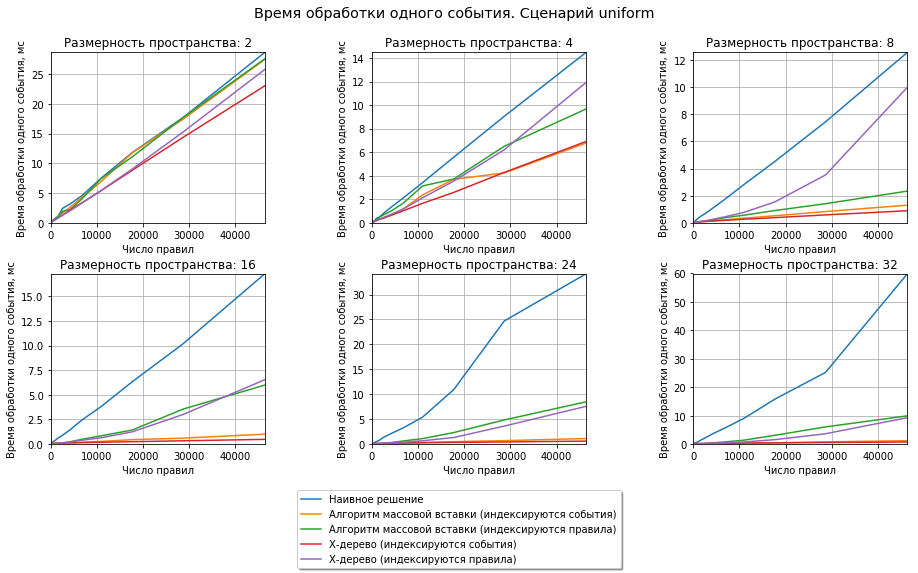
\includegraphics[width=1\textwidth]{images/uniformTime.png}    \includegraphics[width=1\textwidth]{images/uniformSpeedUp.png}
    \caption{Результаты для сценария uniform.}
    \label{fig:uniform}
\end{figure}
\begin{figure}[p]
    \centering
    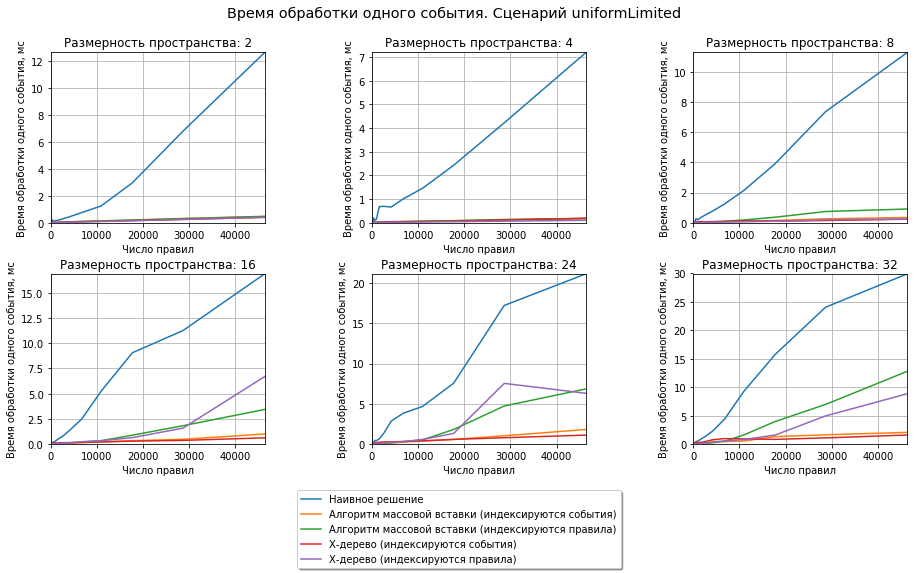
\includegraphics[width=1\textwidth]{images/uniformLimitedTime.png}    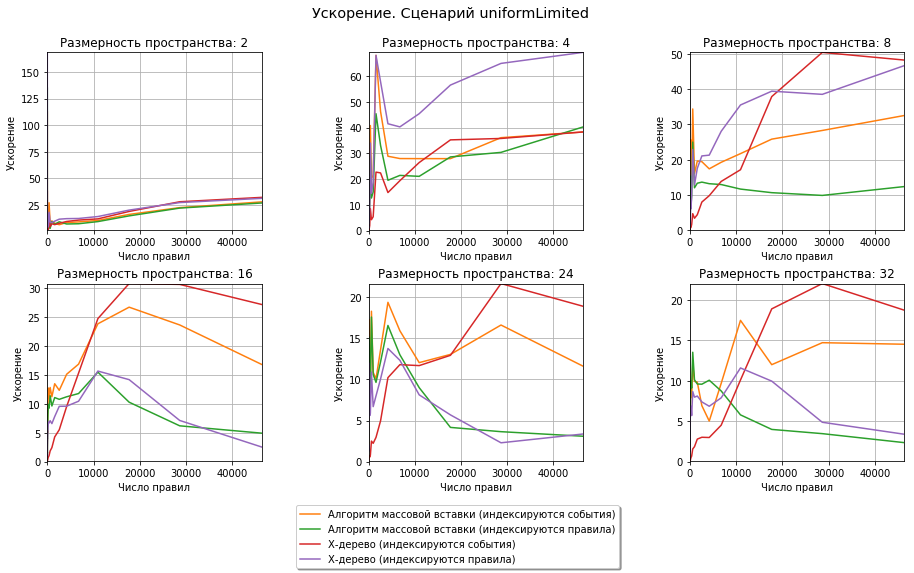
\includegraphics[width=1\textwidth]{images/uniformLimitedSpeedUp.png}
    \caption{Результаты для сценария uniformLimited.}
    \label{fig:uniformLimited}
\end{figure}
\begin{figure}[p]
    \centering
    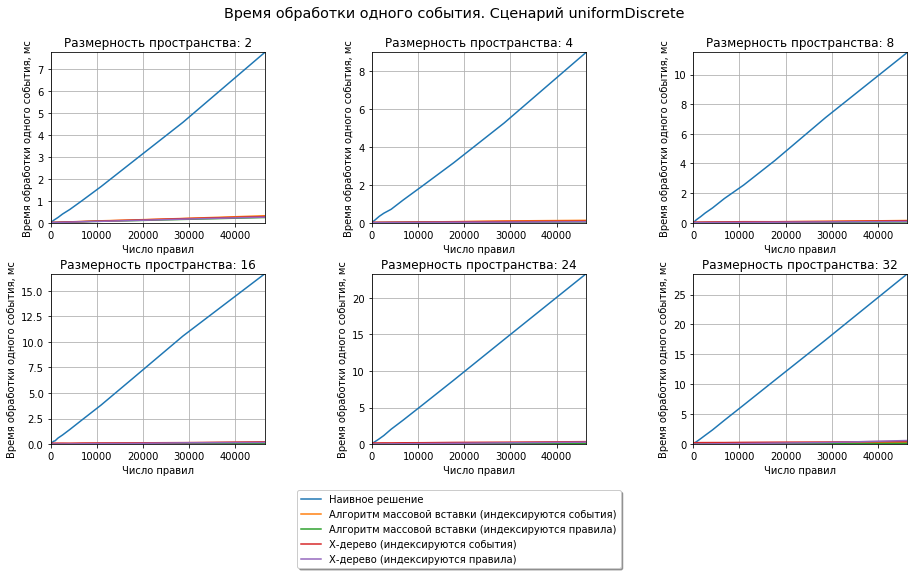
\includegraphics[width=1\textwidth]{images/uniformDiscreteTime.png}    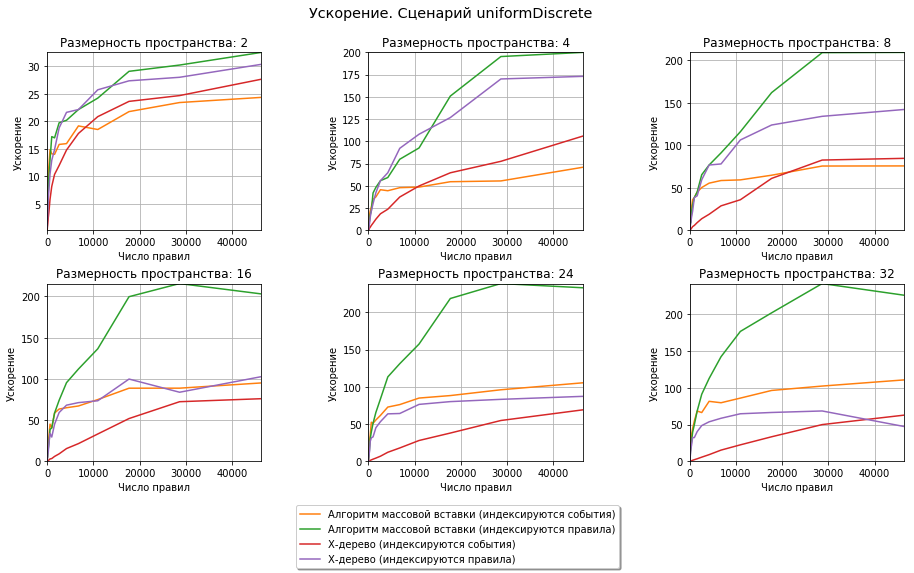
\includegraphics[width=1\textwidth]{images/uniformDiscreteSpeedUp.png}
    \caption{Результаты для сценария uniformDiscrete.}
    \label{fig:uniformDiscrete}
\end{figure}
\begin{figure}[p]
    \centering
    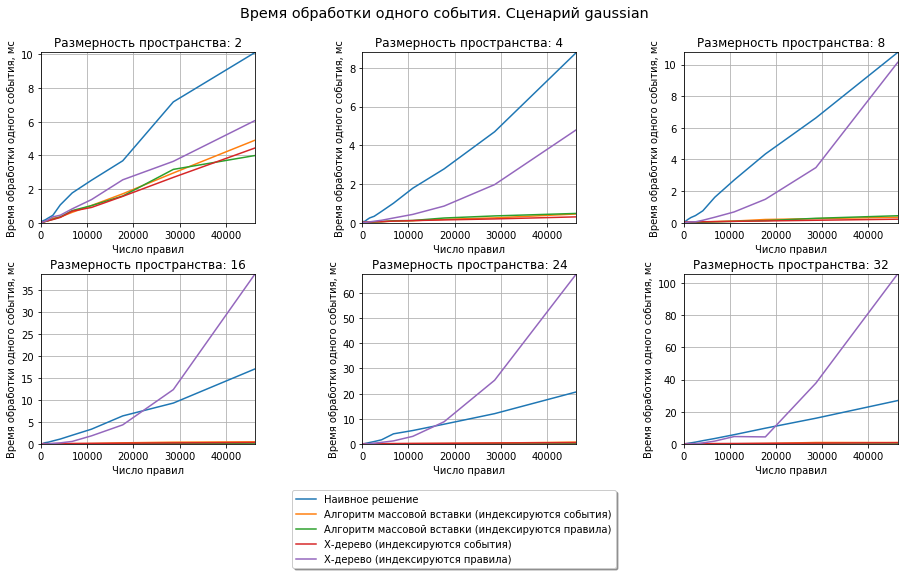
\includegraphics[width=1\textwidth]{images/gaussianTime.png}    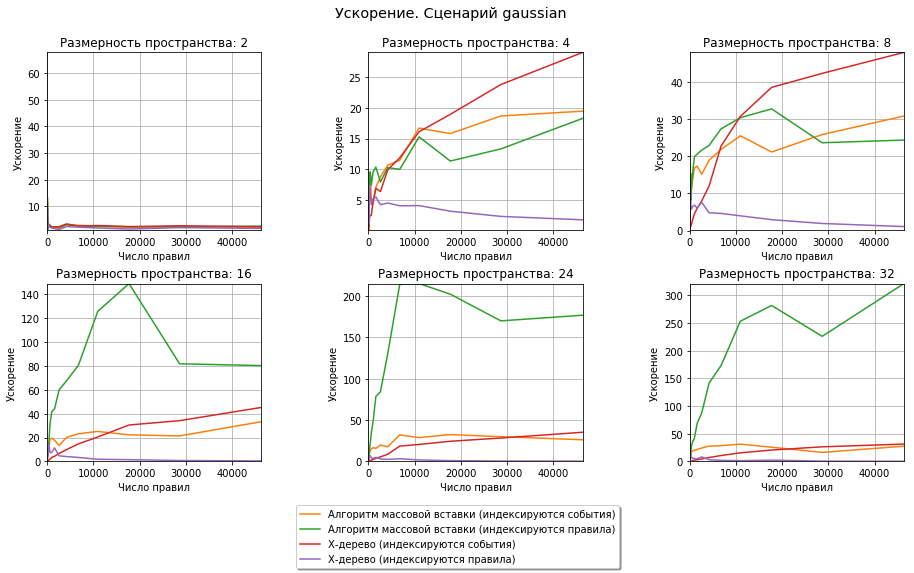
\includegraphics[width=1\textwidth]{images/gaussianSpeedUp.png}
    \caption{Результаты для сценария gaussian.}
    \label{fig:gaussian}
\end{figure}

\subsection{Оптимальный размер группы при индексировании событий}
В главе <<\nameref{section:indexingApproaches}>> описывался подход с индексированием событий. При этом подходе события из входной очереди группируются, для каждой группы строится индекс, и в этом индексе ищутся все правила. Для получения максимальной производительности необходимо подобрать оптимальный размер группы событий.

Для нахождения этого параметра были произведены измерения времени обработки одной точки в зависимости от числа правил и размера группы. Измерения проводились в пространстве размерности 16.

Результаты измерений представлены на рисунке~\ref{fig:pointScript}. По горизонтали отложен размер группы, по вертикали --- число правил. Цветом показана относительная производительность: единица означает наибольшее время работы для фиксированного числа правил и изображена красным цветом; чем ближе цвет к зеленому цвет, тем меньше отношение времени работы к наибольшему времени работы.

По графику заметно: чем больше размер группы, тем эффективнее работает индекс. Для наиболее быстрой обработки необходимо использовать наибольший размер группы, который позволит оперативная память.

\begin{figure}[h!]
    \centering
    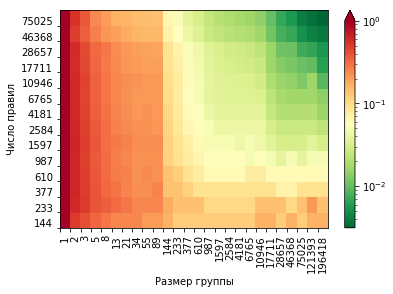
\includegraphics[width=0.75\textwidth]{images/pointScript.png}
    \caption{Относительное время работы в зависимости от числа правил и размера группы.}
    \label{fig:pointScript}
\end{figure}

\subsection{Результаты тестирования системы}
\subsubsection{Тестирование пропускной способности}
Для каждого из сценариев была протестирована пропускная способность для наивного решения и для индекса, оказавшегося наиболее производительным при тестировании в главе~\ref{section:indexTestingResults}. Тестирование проводилось для 8 измерений, 200~000 правил и 4 экземпляров приложения индекса с размером группы 2. Данные были получены с помощью Grafana из метрик, которые отдавало приложение для поиска совпадений. Пропускная способность рассчитывалась как среднее число обработанных событий за промежуток времени среди всех групп деленное на этот промежуток времени. Аналогично рассчитывалась пропускная способность для совпадений. Входное количество событий в единицу времени было больше, чем могла обработать система, чтобы она работала с максимально возможной пропускной способностью. Правила заново запрашивались из базы каждые 10 минут. Измерения производились для интервала в 20 минут.

\paragraph{Сценарий uniform (рисунок~\ref{fig:uniformComposite}).} В данном сценарии пропускные способности индекса и наивного решения близки и равен порядка 30 событий в секунду. Это вызвано тем, что при использовании сценария \verb|uniform| возникает множество совпадений. В данном случае производительность ограничивается скоростью записи совпадений в выходную очередь, а не скоростью поиска совпадений. Для решения этой проблемы нужно увеличить число групп, чтобы на один экземпляр индекса приходилось меньше правил.

\begin{figure}[h!]
    \centering
    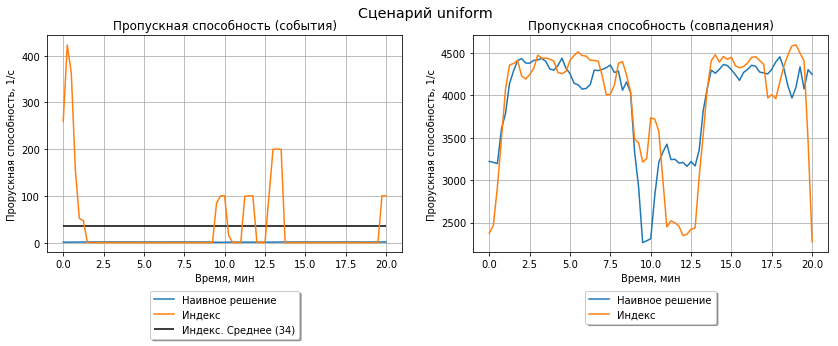
\includegraphics[width=1\textwidth]{images/composite/uniformComposite.png}
    \caption{Пропускная способность системы для сценария uniform.}
    \label{fig:uniformComposite}
\end{figure}

График пропускной способности для событий для индекса имеет несколько пиков, а на остальных участках равен нулю. Это вызвано тем, что для поиска совпадений используется индексирование событий. В момент пика на графике события читаются из входной очереди. В промежуток нулевой пропускной способности по событиям строится дерево, в индексе ищутся правила, и совпадения записываются в выходную очередь.


\paragraph{Сценарий uniformLimited (рисунок~\ref{fig:uniformLimitedComposite}).} В данном сценарии пропускная способность индекса примерно равна 1000 событиям в секунду. Она превышает пропускную способность наивного решения в 20-30 раз.

\begin{figure}[h!]
    \centering
    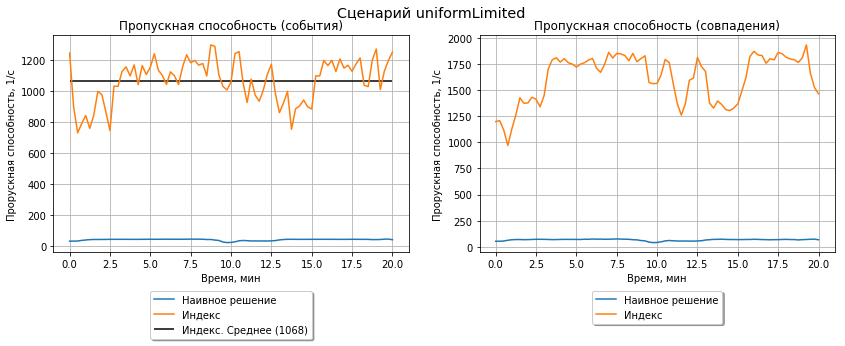
\includegraphics[width=1\textwidth]{images/composite/uniformLimitedComposite.png}
    \caption{Пропускная способность системы для сценария uniformLimited.}
    \label{fig:uniformLimitedComposite}
\end{figure}

\paragraph{Сценарий uniformDiscrete (рисунок~\ref{fig:uniformDiscreteComposite}).} Пропускная способность индекса находится в районе 3000 событий в секунду. Ускорение по сравнению с наивным решением достигает 60 раз.

\begin{figure}[h!]
    \centering
    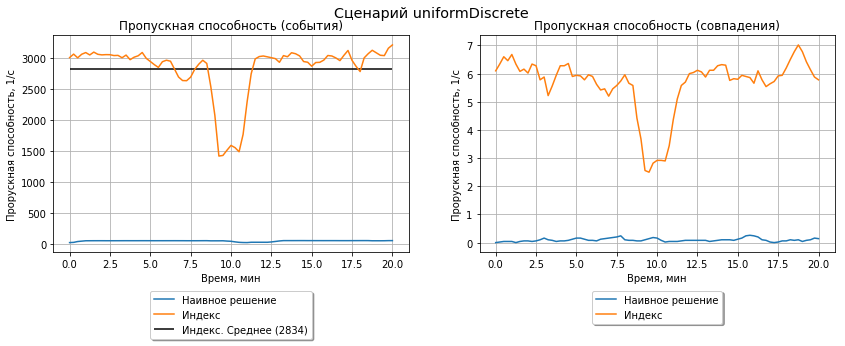
\includegraphics[width=1\textwidth]{images/composite/uniformDiscreteComposite.png}
    \caption{Пропускная способность системы для сценария uniformDiscrete.}
    \label{fig:uniformDiscreteComposite}
\end{figure}

\paragraph{Сценарий gaussian (рисунок~\ref{fig:gaussianComposite}).} Пропускная способность индекса примерно равна 2000 событий в секунду. Ускорение достигает 40 раз.

\begin{figure}[h!]
    \centering
    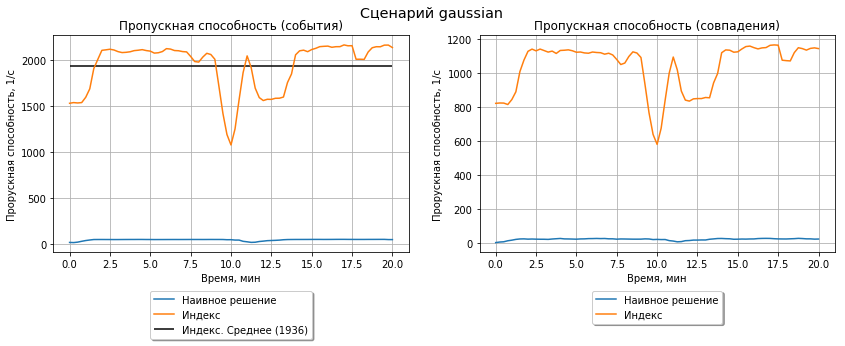
\includegraphics[width=1\textwidth]{images/composite/gaussianComposite.png}
    \caption{Пропускная способность системы для сценария gaussian.}
    \label{fig:gaussianComposite}
\end{figure}

\subsubsection{Тестирование масштабирования}


\section{Выводы}
\subsection{Анализ результатов}
Для решения задачи классификации событий подходят индексы на основе R-деревьев, описанные в данной работе. В зависимости от профиля нагрузки оптимальными будут являться различные виды индексов.

Разработанный прототип системы решает задачу с заданными характеристиками (тысячи событий в секунду и сотни тысяч правил) и масштабируется горизонтально.

\subsection{Дальнейшая работа}
Можно выделить несколько направлений для дальнейшей работы. Они должны улучшить либо расширить функциональность системы.
\begin{itemize}
    \item \emph{Поддержка <<сложных>> правил}. Под <<сложными>> правилами можно понимать конъюнкцию или дизъюнкцию правил, которые использует система. Также среди <<сложных>> правил могут быть правила, в которых задана некоторая зависимость между различными признаками. Такие правила в многомерном пространстве представлялись бы фигурами, отличными от прямоугольников.
    \item \emph{Улучшенный протокол синхронизации}. При использовании разработанного протокола, в моменты изменения числа экземпляров приложения для поиска совпадений, возможно значительное уменьшение пропускной способности системы, так как все индексы должны быть перестроены с нуля. Для решения этой проблемы можно разработать алгоритм, который будет уменьшать число индексов, которые нужно перестроить.
    \item \emph{Динамическое обновление правил}. Для обновления правил в текущей реализации используется механизм кеширования, то есть правила полностью перезапрашиваются из базы данных раз в определенный промежуток времени. Динамическое получение изменений в наборе правил могло бы избавиться от пауз, вызванных перестроением индекса.
\end{itemize}
\newpage

\begin{thebibliography}{9}
\bibitem{flink-use-cases}
Apache Flink Use Cases,\\
\texttt{https://flink.apache.org/usecases.html}.

\bibitem{storm-documentation}
Apache Storm Documentation,\\
\texttt{http://storm.apache.org/index.html}

\bibitem{samza-streams-api}
Apache Samza Streams API,\\
\texttt{https://samza.apache.org/learn/documentation/latest/api/\\high-level-api.html}

\bibitem{mysql-spatial}
MySQL Spatial Types,\\
\texttt{https://dev.mysql.com/doc/refman/8.0/en/spatial-types.html}

\bibitem{postgis}
PostGIS Manual,\\
\texttt{https://postgis.net/docs/manual-3.0/}

\bibitem{oracle-spatial}
Oracle Spatial Features,\\
\texttt{https://www.oracle.com/database/technologies/\\spatialandgraph/spatial-features.html}

\bibitem{r-tree}
Antonin Guttman. \textit{R-Trees: A Dynamic Index Structure for Spatial Searching}. Proc. 1984 ACM SIGMOD International Conference on Management of Data: 47–57.

\bibitem{x-tree}
Stefan Berchtold; Daniel A. Keim; Hans-Peter Kriegel. \textit{The X-tree: An Index Structure for High-Dimensional Data}. Proc. 22nd VLDB Conference. Mumbai, India: 28–39.

\bibitem{r-star-tree}
Norbert Beckmann; Hans-Peter Kriegel; Ralf Schneider; Bernhard Seeger. \textit{The R*-tree: an efficient and robust access method for points and rectangles}. Proc. 1990 ACM SIGMOD International Conference on Management of Data: 322-331.

\bibitem{str}
Scott T. Leutenegger; Mario A. Lopez; Jeffrey Edgington. \textit{STR: A Simple and Efficient Algorithm for R-Tree Packing}. Proc. 1997. 13th IEEE Conference on Data Engineering: 495-506.

\bibitem{omt}
Taewon Lee; Sukho Lee. \textit{OMT: Overlap Minimizing Top-down Bulk Loading Algorithm for R-tree}. 2003. CAiSE Short Paper Proceedings.

\bibitem{kafka}
Apache Kafka Documentation,\\
\texttt{https://kafka.apache.org/documentation/}.

\bibitem{zookeeper}
Apache ZooKeeper Documentation,\\
\texttt{https://zookeeper.apache.org/doc/r3.6.1/index.html}

\bibitem{curator}
Apache Curator Recipes,\\
\texttt{https://curator.apache.org/curator-recipes/index.html}

\bibitem{mongo}
MongoDB Manual,\\
\texttt{https://docs.mongodb.com/manual/}

\bibitem{scala}
Scala Documentation,\\
\texttt{https://docs.scala-lang.org/}

\bibitem{prometheus}
Prometheus Documentation,\\
\texttt{https://prometheus.io/docs}

\bibitem{grafana}
Grafana Documentation,\\
\texttt{https://grafana.com/docs/grafana/latest/}

\bibitem{docker}
Docker Documentation,\\
\texttt{https://docs.docker.com/}

\bibitem{zio}
ZIO documentation,\\
\texttt{https://zio.dev/docs/overview/overview\_index}

\bibitem{fs2}
Functional Steams For Scala Guide,\\
\texttt{https://fs2.io/guide.html}

\bibitem{protobuf}
ProtocolBuffers Documentation,\\
\texttt{https://developers.google.com/protocol-buffers}

\bibitem{uuid}
\textit{A Universally Unique IDentifier (UUID) URN Namespace},
RFC-4122,\\
\texttt{https://tools.ietf.org/html/rfc4122}

\end{thebibliography}
\end{document}
